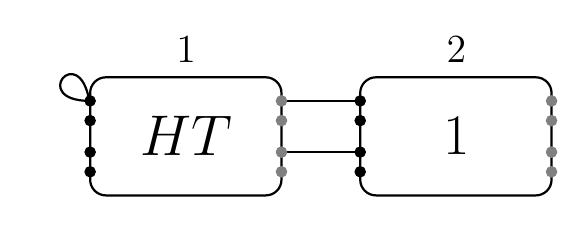
\begin{tikzpicture}
  % The connections 
 \foreach \y in {1.2,.55}
{   
 \draw[thick] (2.43,\y) -- (3.43,\y);  
}      
\draw[thick,looseness = 200] (0,1.2) to [out = 180, in = 100] (-.01,1.2);
  % The two rectangles 
 \foreach \offset/\unitary/\label in {0/HT/1,3.43/1/2}
{ 
 \begin{scope}[xshift=\offset cm] 
 \draw[rounded corners=2mm,thick] (0,0) rectangle (2.43cm,1.5 cm);
 \foreach \x /\color in {0/black,2.43/gray}
{     
\foreach \y in {1.2,.95,.55,.3}
{      
\draw[fill=\color,draw=\color] (\x cm, \y cm) circle (.66mm);  
  }
}    
\node at (1.22cm, .75cm) {\huge $\unitary$};   
 \node at (1.22cm, 1.85cm){\Large \label};  
\end{scope}
}    
\end{tikzpicture}